\documentclass[]{article}

% ------
% Fonts and typesetting settings
\usepackage[sc]{mathpazo}
\usepackage[T1]{fontenc}
\linespread{1.05} % Palatino needs more space between lines
\usepackage{microtype}
\usepackage{amsmath}

% ------
% Page layout
\usepackage[hmarginratio=1:1,top=30mm,bottom=30mm,columnsep=20pt]{geometry}
\usepackage[font=it]{caption}
\usepackage{paralist}
%\usepackage{multicol}

\usepackage{graphicx}
\usepackage{color}
\usepackage{tabularx}

%\usepackage{wrapfig}

\usepackage{capt-of}

% \usepackage[ngerman]{babel}

% ------
% Lettrines
\usepackage{lettrine}

% ------
% Abstract
\usepackage{abstract}
	\renewcommand{\abstractnamefont}{\normalfont\bfseries}
	\renewcommand{\abstracttextfont}{\normalfont\small\itshape}


% ------
% Titling (section/subsection)
\usepackage{titlesec}
\renewcommand\thesection{\Roman{section}}
\titleformat{\section}[block]{\large\scshape\centering}{\thesection.}{1em}{}


% ------
% Header/footer
\usepackage{fancyhdr}
	\pagestyle{fancy}
	\fancyhead{}
	\fancyfoot{}
	\fancyhead[C]{Post-quantum cryptography $\bullet$ Winter 2018/19 $\bullet$ RheinMain University of Applied Sciences}
	\fancyfoot[RO,LE]{\thepage}


% ------
% Maketitle metadata
\title{\vspace{-7mm}%
	\fontsize{24pt}{10pt}\selectfont
	\textbf{Re-implementation of the Picnic signaturescheme in Python}
	}	
\author{%
	\large
	\textsc{Thorsten Knoll} \\[2mm]
	\normalsize	info@thorstenknoll.de \\[2mm]
	\normalsize March, 2019
	%\vspace{-5mm}
	}
\date{}

\usepackage[utf8]{inputenc}

\usepackage{hyperref}

%%%%%%%%%%%%%%%%%%%%%%%%
\begin{document}

\maketitle
\thispagestyle{fancy}

%\begin{abstract}
%\noindent Abstract goes here
%\end{abstract}

\section{Introduction}
\subsection{Post-quantum cryptography, NIST and Picnic}
Quantum computers are experiencing fast development and seem to be available within a timeframe of the next few decades. One of their properties will be to break huge parts of modern cryptography. Especially the discrete logarithm and prime-factorisation loose their trapdoor funcionality in regards to the efficient quantum algorithms from Grover and Shor. Therefore the need for new cryptographic algorithms arises, beeing save in regards to the availability of quantum computers. This field of research goes with the name "Post-quantum cryptography" (PQC). The american National Institute of Standards and Technology (NIST) called out a challenge to find the next PQC standards. This challenge is in round two of three at the time of writing this document. 69 submissions from round one were reduced to 26 candidates in round two of the challenge. These 26 candidates got announced by NIST not long ago at the end of january 2019. One of the submissions surviving the first round is the Picnic signaturescheme.
\subsection{Evaluation and categorization}
\subsection{Learning PQC}
\subsection{Reference documents and implementations by the Picnic Team}
\newpage

\section{LowMC}
\subsection{Idea and overview}
LowMC is a blockcipher in a roundbased construction scheme like many other blockciphers. The name is an abbreviation for "Low multiplicative complexity". XOR in GF2 is a linear operation (ADD), while the multiplication (AND) in GF2 is a non-linear operation (Figure \ref{fig:gates}). LowMC tries to keep the count of AND operations as low as possible while still maintaining a given security level (L1, L3, L5). In Picnic, the low mutliplicative complexity of LowMC is used for reducing the signature lengths. \\
\begin{figure}[htbp]
\center
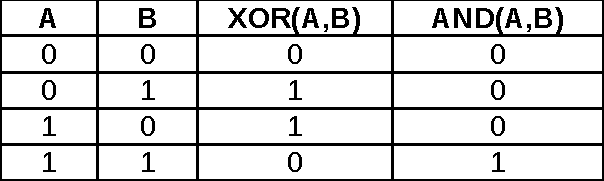
\includegraphics[width=0.4\textwidth]{pics/gates.pdf}
\caption{Linear and non-linear operations}
\label{fig:gates}
\end{figure}\\
Figure \ref{fig:lowmcscheme} shows the roundbased scheme of LowMC. Only the sbox part of the algorithm uses multiplications (ANDs). The other parts strictly contain only linear operations.  
\begin{figure}[htbp]
\center
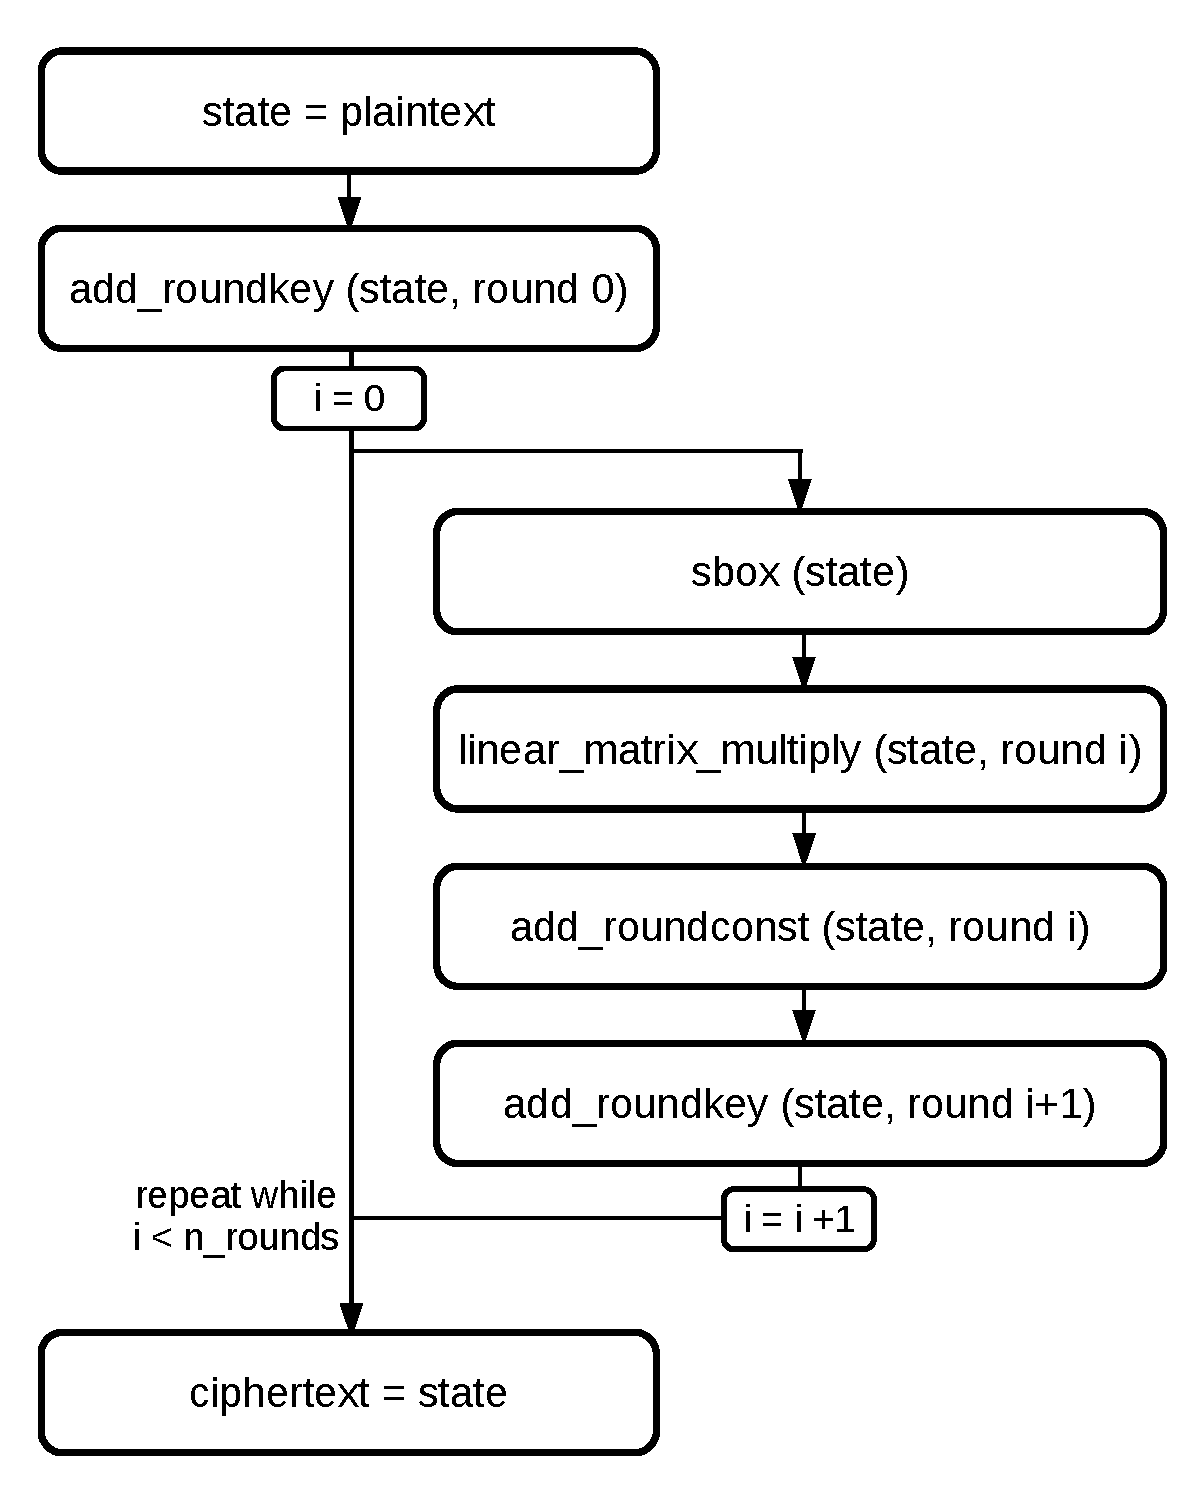
\includegraphics[width=0.55\textwidth]{pics/lowmc_scheme.pdf}
\caption{LowMC scheme}
\label{fig:lowmcscheme}
\end{figure}
\subsection{Pre-calculated constants}
The python program \texttt{generator.py} generates the files for all security levels with the following pre-calculated constants:
\begin{itemize}
\item{Linear layer matrices}
\item{Round constants}
\item{Roundkey matrices}
\end{itemize}
The generation of the constants-files is not mandatory for usage as the project contains them "ready to use". 
\subsection{Private functions}
\subsubsection{\texttt{\_\_apply\_sbox()}}
\subsubsection{\texttt{\_\_multiply\_with\_lin\_mat(round)}}
\subsubsection{\texttt{Add roundconstant}}
\subsubsection{\texttt{\_\_multiply\_with\_lin\_mat(round)}}
\subsubsection{\texttt{Decryption functions}}
\subsection{Public functions (API)}
\subsubsection{\texttt{LowMC(Security level) - Constructor}}
Constrcuts an object of LowMC with the parameters regarding to the security level. The following security levels are available and shall be given to the constructor as strings: "picnic-L1", "picnic-L3" and "picnic-L5". The fitting file with the constants must be in the project directory and gets read (see Pre-calculated constants).
\subsubsection{\texttt{generate\_priv\_key()}}
Generates a private key of the length specified within the security level. The private key is stored in a private variable. The python package CSPRNG \texttt{os.urandom(bytelength)} is used.
\subsubsection{\texttt{set\_priv\_key(priv\_key)}}
Instead of generating the private key it can also be set by giving a bytearry to this function. The bytearray must match the specified keylength from the security level.
\subsubsection{\texttt{encrypt(plaintext)}}
Encrypts a plaintext and returns the ciphertext. The plaintext length must match the specified blocksize length (security level) and must be given as a bytearray to the function. The ciphertext is returned as a bytearray of the same length. Before using this function a private key must be set (or generated).
\subsubsection{\texttt{decrypt(ciphertext)}}
Decrypts a ciphtertext and returns the plaintext. The ciphertext length must match the specified blocksize length (security level) and must be given as a bytearray to the function. The plaintext is returned as a bytearray of the same length. Before using this function a private key must be set (or generated).
\subsection{Testvectors}
\section{Picnic}

\bibliographystyle{unsrt}
\bibliography{}



\end{document}
